\documentclass{standalone}
\usepackage{tikz}
\usetikzlibrary{patterns, positioning}
\usetikzlibrary{shapes.misc}
\usepackage[outline]{contour}
\contourlength{1.5pt} 


\begin{document}
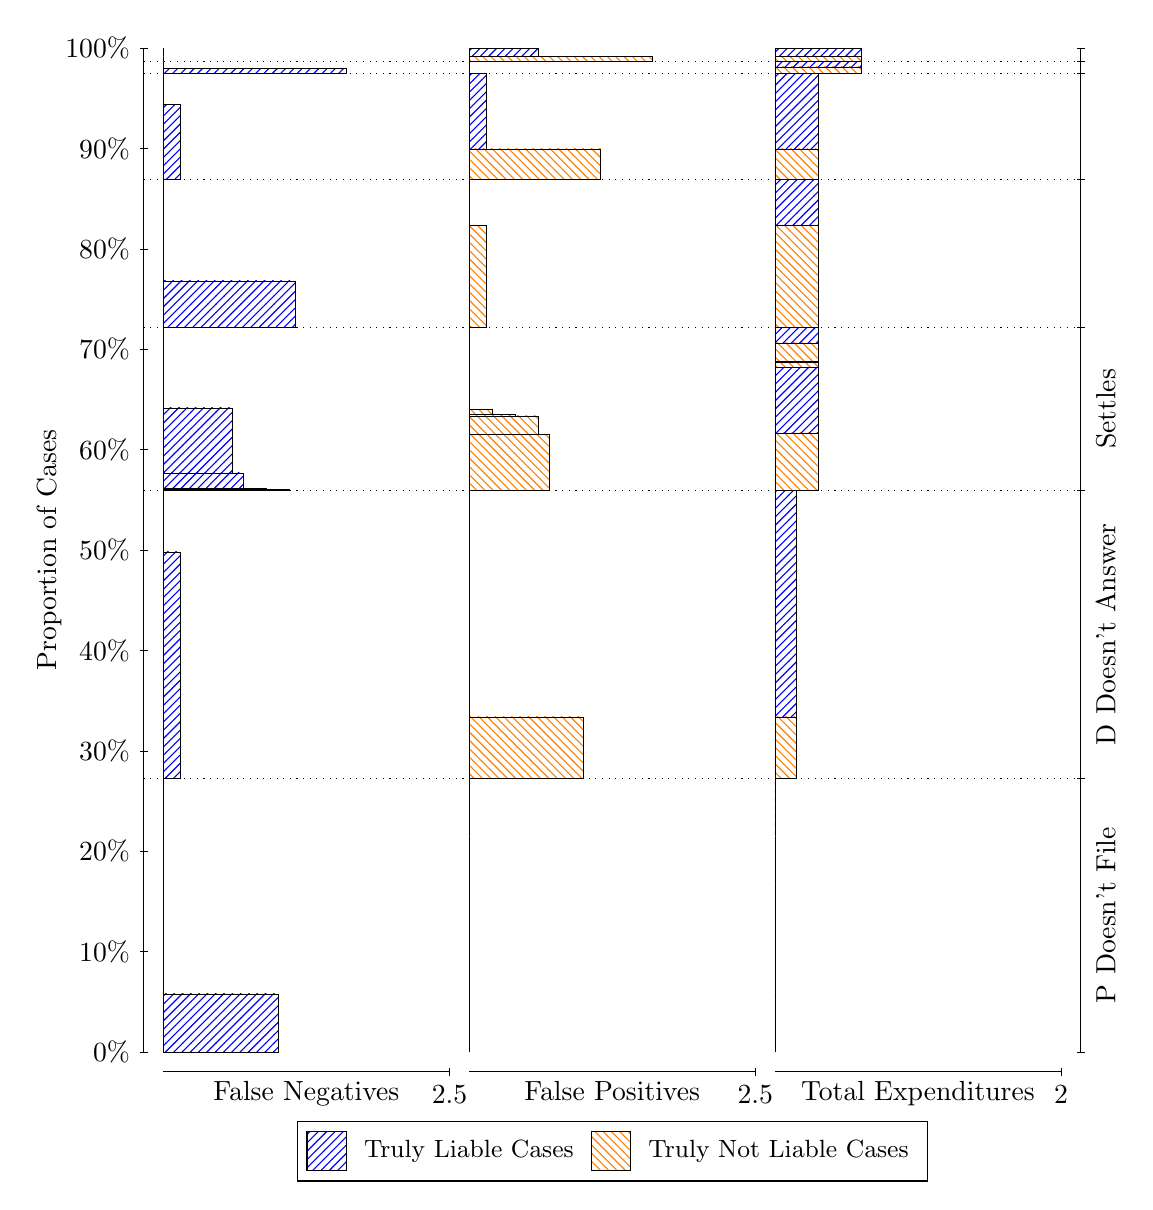
\begin{tikzpicture}
\draw[black, very thin] (1.5,1.75) -- (1.5,14.5);
\node[rotate=90, text=black, anchor=center] at (0.3, 8.125) {Proportion of Cases};
\draw[black, very thin] (1.45,1.75) -- (1.55,1.75);
\node[text=black, anchor=east] at (1.45, 1.75) {0\%};
\draw[black, very thin] (1.45,3.025) -- (1.55,3.025);
\node[text=black, anchor=east] at (1.45, 3.025) {10\%};
\draw[black, very thin] (1.45,4.3) -- (1.55,4.3);
\node[text=black, anchor=east] at (1.45, 4.3) {20\%};
\draw[black, very thin] (1.45,5.575) -- (1.55,5.575);
\node[text=black, anchor=east] at (1.45, 5.575) {30\%};
\draw[black, very thin] (1.45,6.85) -- (1.55,6.85);
\node[text=black, anchor=east] at (1.45, 6.85) {40\%};
\draw[black, very thin] (1.45,8.125) -- (1.55,8.125);
\node[text=black, anchor=east] at (1.45, 8.125) {50\%};
\draw[black, very thin] (1.45,9.4) -- (1.55,9.4);
\node[text=black, anchor=east] at (1.45, 9.4) {60\%};
\draw[black, very thin] (1.45,10.675) -- (1.55,10.675);
\node[text=black, anchor=east] at (1.45, 10.675) {70\%};
\draw[black, very thin] (1.45,11.95) -- (1.55,11.95);
\node[text=black, anchor=east] at (1.45, 11.95) {80\%};
\draw[black, very thin] (1.45,13.225) -- (1.55,13.225);
\node[text=black, anchor=east] at (1.45, 13.225) {90\%};
\draw[black, very thin] (1.45,14.5) -- (1.55,14.5);
\node[text=black, anchor=east] at (1.45, 14.5) {100\%};

\draw[black, very thin] (13.4,1.75) -- (13.4,14.5);
\draw[black, very thin] (13.35,1.75) -- (13.45,1.75);
\node[anchor=west] at (13.35, 1.75) {};
\draw[black, very thin] (13.35,5.226) -- (13.45,5.226);
\node[anchor=west] at (13.35, 5.226) {};
\draw[black, very thin] (13.35,8.8798) -- (13.45,8.8798);
\node[anchor=west] at (13.35, 8.8798) {};
\draw[black, very thin] (13.35,10.956) -- (13.45,10.956);
\node[anchor=west] at (13.35, 10.956) {};
\draw[black, very thin] (13.35,12.833) -- (13.45,12.833);
\node[anchor=west] at (13.35, 12.833) {};
\draw[black, very thin] (13.35,14.173) -- (13.45,14.173);
\node[anchor=west] at (13.35, 14.173) {};
\draw[black, very thin] (13.35,14.326) -- (13.45,14.326);
\node[anchor=west] at (13.35, 14.326) {};
\draw[black, very thin] (13.35,14.5) -- (13.45,14.5);
\node[anchor=west] at (13.35, 14.5) {};

\draw[black, very thin, pattern color=blue, pattern=north east lines] (1.75,1.75) rectangle (3.2033,2.4874);
\draw[black, very thin, pattern color=orange, pattern=north west lines] (1.75,2.4874) rectangle (1.75,5.226);
\draw[black, very thin, pattern color=blue, pattern=north east lines] (1.75,5.226) rectangle (1.968,8.1009);
\draw[black, very thin, pattern color=orange, pattern=north west lines] (1.75,8.1009) rectangle (1.75,8.8798);
\draw[black, very thin, pattern color=blue, pattern=north east lines] (1.75,8.8798) rectangle (3.3487,8.8937);
\draw[black, very thin, pattern color=blue, pattern=north east lines] (1.75,8.8937) rectangle (3.058,8.9048);
\draw[black, very thin, pattern color=blue, pattern=north east lines] (1.75,8.9048) rectangle (2.7673,9.1057);
\draw[black, very thin, pattern color=blue, pattern=north east lines] (1.75,9.1057) rectangle (2.622,9.9295);
\draw[black, very thin, pattern color=orange, pattern=north west lines] (1.75,9.9295) rectangle (1.75,10.956);
\draw[black, very thin, pattern color=blue, pattern=north east lines] (1.75,10.956) rectangle (3.4213,11.543);
\draw[black, very thin, pattern color=orange, pattern=north west lines] (1.75,11.543) rectangle (1.75,12.833);
\draw[black, very thin, pattern color=blue, pattern=north east lines] (1.75,12.833) rectangle (1.968,13.788);
\draw[black, very thin, pattern color=orange, pattern=north west lines] (1.75,13.788) rectangle (1.75,14.173);
\draw[black, very thin, pattern color=blue, pattern=north east lines] (1.75,14.173) rectangle (4.0753,14.238);
\draw[black, very thin, pattern color=orange, pattern=north west lines] (1.75,14.238) rectangle (1.75,14.326);
\draw[black, very thin, pattern color=orange, pattern=north west lines] (1.75,14.326) rectangle (1.75,14.395);
\draw[black, very thin, pattern color=blue, pattern=north east lines] (1.75,14.395) rectangle (1.75,14.5);
\draw[black, very thin, pattern color=orange, pattern=north west lines] (5.6333,1.75) rectangle (5.6333,4.4886);
\draw[black, very thin, pattern color=blue, pattern=north east lines] (5.6333,4.4886) rectangle (5.6333,5.226);
\draw[black, very thin, pattern color=orange, pattern=north west lines] (5.6333,5.226) rectangle (7.0867,6.0049);
\draw[black, very thin, pattern color=blue, pattern=north east lines] (5.6333,6.0049) rectangle (5.6333,8.8798);
\draw[black, very thin, pattern color=orange, pattern=north west lines] (5.6333,8.8798) rectangle (6.6507,9.59);
\draw[black, very thin, pattern color=orange, pattern=north west lines] (5.6333,9.59) rectangle (6.5053,9.8282);
\draw[black, very thin, pattern color=orange, pattern=north west lines] (5.6333,9.8282) rectangle (6.2147,9.8503);
\draw[black, very thin, pattern color=orange, pattern=north west lines] (5.6333,9.8503) rectangle (5.924,9.9062);
\draw[black, very thin, pattern color=blue, pattern=north east lines] (5.6333,9.9062) rectangle (5.6333,10.956);
\draw[black, very thin, pattern color=orange, pattern=north west lines] (5.6333,10.956) rectangle (5.8513,12.246);
\draw[black, very thin, pattern color=blue, pattern=north east lines] (5.6333,12.246) rectangle (5.6333,12.833);
\draw[black, very thin, pattern color=orange, pattern=north west lines] (5.6333,12.833) rectangle (7.3047,13.218);
\draw[black, very thin, pattern color=blue, pattern=north east lines] (5.6333,13.218) rectangle (5.8513,14.173);
\draw[black, very thin, pattern color=orange, pattern=north west lines] (5.6333,14.173) rectangle (5.6333,14.261);
\draw[black, very thin, pattern color=blue, pattern=north east lines] (5.6333,14.261) rectangle (5.6333,14.326);
\draw[black, very thin, pattern color=orange, pattern=north west lines] (5.6333,14.326) rectangle (7.9587,14.395);
\draw[black, very thin, pattern color=blue, pattern=north east lines] (5.6333,14.395) rectangle (6.5053,14.5);
\draw[black, very thin, pattern color=orange, pattern=north west lines] (9.5167,1.75) rectangle (9.5167,4.4886);
\draw[black, very thin, pattern color=blue, pattern=north east lines] (9.5167,4.4886) rectangle (9.5167,5.226);
\draw[black, very thin, pattern color=orange, pattern=north west lines] (9.5167,5.226) rectangle (9.7892,6.0049);
\draw[black, very thin, pattern color=blue, pattern=north east lines] (9.5167,6.0049) rectangle (9.7892,8.8798);
\draw[black, very thin, pattern color=orange, pattern=north west lines] (9.5167,8.8798) rectangle (10.062,9.6122);
\draw[black, very thin, pattern color=blue, pattern=north east lines] (9.5167,9.6122) rectangle (10.062,10.447);
\draw[black, very thin, pattern color=orange, pattern=north west lines] (9.5167,10.447) rectangle (10.062,10.503);
\draw[black, very thin, pattern color=blue, pattern=north east lines] (9.5167,10.503) rectangle (10.062,10.517);
\draw[black, very thin, pattern color=orange, pattern=north west lines] (9.5167,10.517) rectangle (10.062,10.755);
\draw[black, very thin, pattern color=blue, pattern=north east lines] (9.5167,10.755) rectangle (10.062,10.956);
\draw[black, very thin, pattern color=orange, pattern=north west lines] (9.5167,10.956) rectangle (10.062,12.246);
\draw[black, very thin, pattern color=blue, pattern=north east lines] (9.5167,12.246) rectangle (10.062,12.833);
\draw[black, very thin, pattern color=orange, pattern=north west lines] (9.5167,12.833) rectangle (10.062,13.218);
\draw[black, very thin, pattern color=blue, pattern=north east lines] (9.5167,13.218) rectangle (10.062,14.173);
\draw[black, very thin, pattern color=orange, pattern=north west lines] (9.5167,14.173) rectangle (10.607,14.261);
\draw[black, very thin, pattern color=blue, pattern=north east lines] (9.5167,14.261) rectangle (10.607,14.326);
\draw[black, very thin, pattern color=orange, pattern=north west lines] (9.5167,14.326) rectangle (10.607,14.395);
\draw[black, very thin, pattern color=blue, pattern=north east lines] (9.5167,14.395) rectangle (10.607,14.5);
\draw[black, dotted] (1.5,5.226) -- (13.4,5.226);
\draw[black, dotted] (1.5,8.8798) -- (13.4,8.8798);
\draw[black, dotted] (1.5,10.956) -- (13.4,10.956);
\draw[black, dotted] (1.5,12.833) -- (13.4,12.833);
\draw[black, dotted] (1.5,14.173) -- (13.4,14.173);
\draw[black, dotted] (1.5,14.326) -- (13.4,14.326);
\draw[black, very thin] (1.75,1.5) -- (5.3833,1.5);
\node[text=black, anchor=north] at (3.5667, 1.5) {False Negatives};
\draw[black, very thin] (5.3833,1.45) -- (5.3833,1.55);
\node[text=black, anchor=north] at (5.3833, 1.45) {2.5};

\draw[black, very thin] (5.6333,1.5) -- (9.2667,1.5);
\node[text=black, anchor=north] at (7.45, 1.5) {False Positives};
\draw[black, very thin] (9.2667,1.45) -- (9.2667,1.55);
\node[text=black, anchor=north] at (9.2667, 1.45) {2.5};

\draw[black, very thin] (9.5167,1.5) -- (13.15,1.5);
\node[text=black, anchor=north] at (11.333, 1.5) {Total Expenditures};
\draw[black, very thin] (13.15,1.45) -- (13.15,1.55);
\node[text=black, anchor=north] at (13.15, 1.45) {2};

\node[text=black, centered, rotate=90] at (13.72, 3.488) {\contour{white}{P Doesn't File}};
\node[text=black, centered, rotate=90] at (13.72, 7.0529) {\contour{white}{D Doesn't Answer}};
\node[text=black, centered, rotate=90] at (13.72, 9.9179) {\contour{white}{Settles}};





\draw (7.449999999999999,1.5) node[draw=none] (baseCoordinate) {};
\begin{scope}[align=center]
        \matrix[scale=0.5, draw=black, below=0.5cm of baseCoordinate, nodes={draw}, column sep=0.1cm]{
            \node[rectangle, draw, minimum width=0.5cm, minimum height=0.5cm, pattern color=blue, pattern=north east lines] {}; &
            \node[draw=none, font=\small, text=black] (B) {Truly Liable Cases}; &
            \node[rectangle, draw, minimum width=0.5cm, minimum height=0.5cm, pattern color=orange, pattern=north west lines] {}; &
            \node[draw=none, font=\small, text=black] (B) {Truly Not Liable Cases}; \\
            };
\end{scope}

\end{tikzpicture}
\end{document}